\chapter{Introduction}
    This document was created as a report about the project. The project is part of the Master's program in Business Informatics at HTW Berlin. The project has been presented by DATANOMIQ GmbH and was accompanied by Signavio GmbH as a cooperation partner.

    \section{Background}
    As a part of business intelligence, process mining is a way for modern companies to get information about their processes. It is not uncommon for processes to be further adapted and changed over time. The question always arises to what extent the changes have influenced the measurement results of the process.

    \section{Goal}
    In order to specify this question further, it should be found out whether there is a causal relationship between the change in the process and the change in the measurement result. In the best case, the goal is to find the specific changes from all the changes that also influence the measurement result.

    \section{Structure}
    First, the methods used are introduced. This is to clarify afterwards, for which reasons which kind of data was used. Afterwards, the implementation of the software will be discussed in order to explain its peculiarities, limitations and possibilities.

\clearpage
%- - - - - - - - - - - - - - - - - - - - - - - - - - - - - - - - - - - - - - - - - - - - - - - - - - - - - - -
\chapter{Double Machine Learning}

    \section{In general}
    A data-based causal analysis attempts to measure the effect of a change on observable outcome. The measurement of this effect is possible when the changes are observable. This can be implemented by double machine learning. In general, it tries to estimate the effect of the change on the outcome by the changes.\footcite[see][106]{mahu2020} In order to recognize the causal effect of a change, all other influences must be comparable.\footcite[see][107]{mahu2020} In addition, it is necessary that the results can arise from the same characteristics, as well as there should be no combination that is found only before the change or after the change.\footcite[see][109]{mahu2020}\\
    By using machine learning, the relationships between the changes and their effects can be represented as machine models. It should be noted that the representation as a model is always only an approximately correct estimate of the real relationship.\footcite[see][111]{mahu2020}Now we can assume that there are two models. One to calculate the result under condition of the change and one to explain the change. By assuming that a change is calculable if the calculation of the first model is different under the different conditions (changed/not changed), it can be assumed that the representation of the change by the second model explains the difference.\footcite[see][112\psqq]{mahu2020}

    \section{In this case}
    In this case, however, we are talking about process changes. If there is a suitable representation of the process properties in the flow and its results, then double machine learning can also be used for this. In the following, the idea is explained with an example.
    \begin{figure}[H]
        \centering
        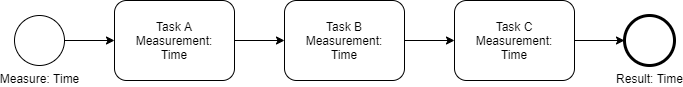
\includegraphics[width=0.99\textwidth-2\fboxsep-2\fboxrule]{includes/p1.png}
        \caption{Process 1 (Unchanged)}
        \label{p1}
    \end{figure}
    \begin{figure}[H]
        \centering
        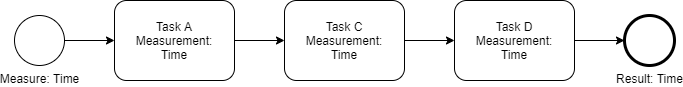
\includegraphics[width=0.99\textwidth-2\fboxsep-2\fboxrule]{includes/p2.png}
        \caption{Process 2 (Changed)}
        \label{p2}
    \end{figure}
    As can be seen in the figures, Task B was deleted and Task D was introduced in the modified process. As a simple example, we now use time as our measurand. Here, the result of the measurement is the sum of the time used for the tasks. We can therefore set up the following example functions:\\
    \small{$p_1$/$p_2$ representing the results, $A$..$D$ representing the measurements}
    \[p_1 = A + B + C\]
    \[p_2 = A + C + D\]
    Now, we can assume that a machine learning model ($u$) can be trained for the unmodified process as the adornment of the estimate p1 and as the characteristics A..C. Then, we can try to use the model ($u$) to perform a prediction for our modified process to measure the difference ($\beta$) in the outcome.
    \[u \approx p_1\]
    However, this requires the model to make a prediction ($q$) for the outcome of the changed process.
    \[u \rightarrow p_2 \approx q\]
    Now the difference ($\beta$) can be calculated.
    \[\beta = p_2 - q\]
    A second model ($m$) shows the effect of the change on the difference.
    \[m \approx \beta\]
    In this case, it is clear because the change in results can only be explained by task D.
    \[m \equiv D\]
    In more complex examples, it is conceivable that the change in difference may also consist of combination of changed characteristics. In the end, it is only necessary to find out whether the estimation of the difference was successful. A classical regressive measurement would be the mean squared error. The smaller this is (closer to zero) the better the estimation succeeds and thus the presentation as a causal reason.
    \[m \rightarrow \beta \equiv \beta_m\]
    \[causality = mean((\beta-\beta_m)^2)\]
\clearpage
%- - - - - - - - - - - - - - - - - - - - - - - - - - - - - - - - - - - - - - - - - - - - - - - - - - - - - - -
\chapter{Data acquisition}

    \section{Real Data}
    To implement such an algorithm, you need data to work with. In the best case, real data is available from a company that has just adapted its processes. The difficulty is that there must be at least two data sets from the same process. One must represent the state before the changes and one after the changes.\\
    Since no data could be provided during the course of the project, some had to be sought. One place to start is the Business Process Intelligence Challenge, which annually challenges participants with problems in process mining. However, even after finding two data sets, with the same origin and the same process, problems arose. On the one hand, the datasets were in different languages and on the other hand, some of them were poorly described. This is due to the time gap of five years (2012\footnote{BPI 2012 https://www.win.tue.nl/bpi/doku.php?id=2012:challenge}, 2017\footnote{BPI 2017 https://www.win.tue.nl/bpi/doku.php?id=2017:challenge}). Therefore, it was decided to simulate data.

    \section{Simulation}
    During the project, a simple order-to-cash process was designed in BPMN-format. The order-to-cash process encompasses all steps from when a customer order is placed up until the business is paid (the cash). Those steps include order management and order fulfillment, through to credit management, then invoicing and ultimately payment collection. Since the project does not focus on developing a complex process, a simplified process was used.\\
    A variety of sources were consulted for this purpose and finally the process from the following source was used: \cite[][373]{madu2018}.\\
    Other processes from \cite[][251]{dafi2020} and \cite[][353]{duer2017} were under consideration, but were discarded as the project progressed.\\
    The BPMN process shows the process from ordering a product to delivery. The example company works with two suppliers. The three roles of the ERP system, a warehouse employee and a sales employee are represented by swin lanes. When a customer orders a product, it is checked whether it is already in stock. If it is, the product is ordered from the warehouse and confirmed after the order is received. If the product is not in stock, the raw materials are ordered from the two suppliers and then the product is manufactured. If the product is then available, the product is shipped to the customer's delivery address. At the same time, an invoice is sent to the customer. When the amount is received and the product has been delivered, the order is archived, and the process is finished.\\    
    The process is considered the basis for the project. For this purpose, a second similar process will be developed, in which the first process will be modified.\\
    The BPMN process can be found on the next page.
    \begin{figure}[H]
        \centering
        \fbox{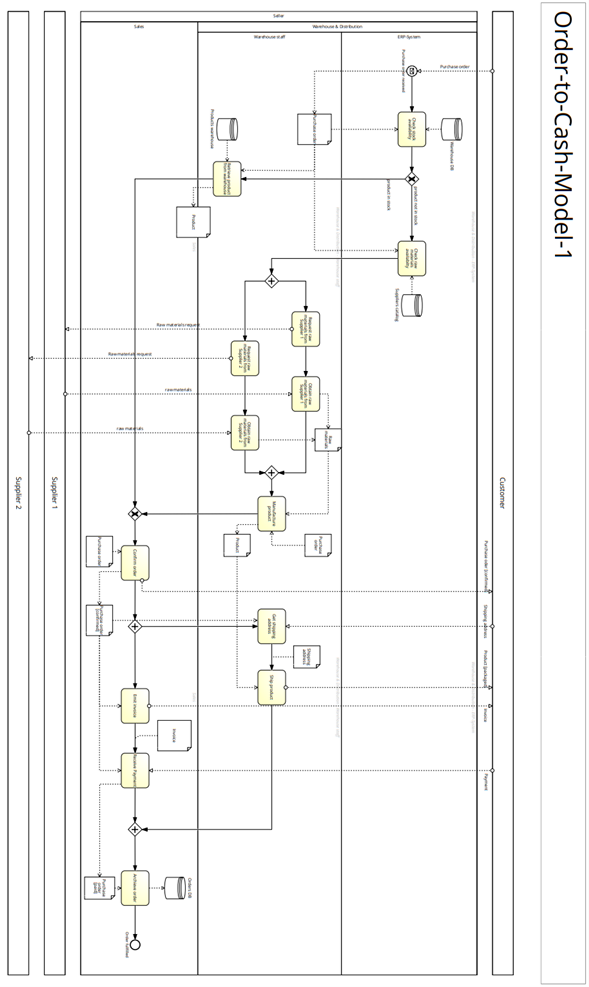
\includegraphics[height=23cm]{includes/p1_bpmn.png}}
        \caption{BPMN: Process 1 (Unchanged)}
        \label{bpmn1}
    \end{figure}
    \begin{figure}[H]
        \centering
        \fbox{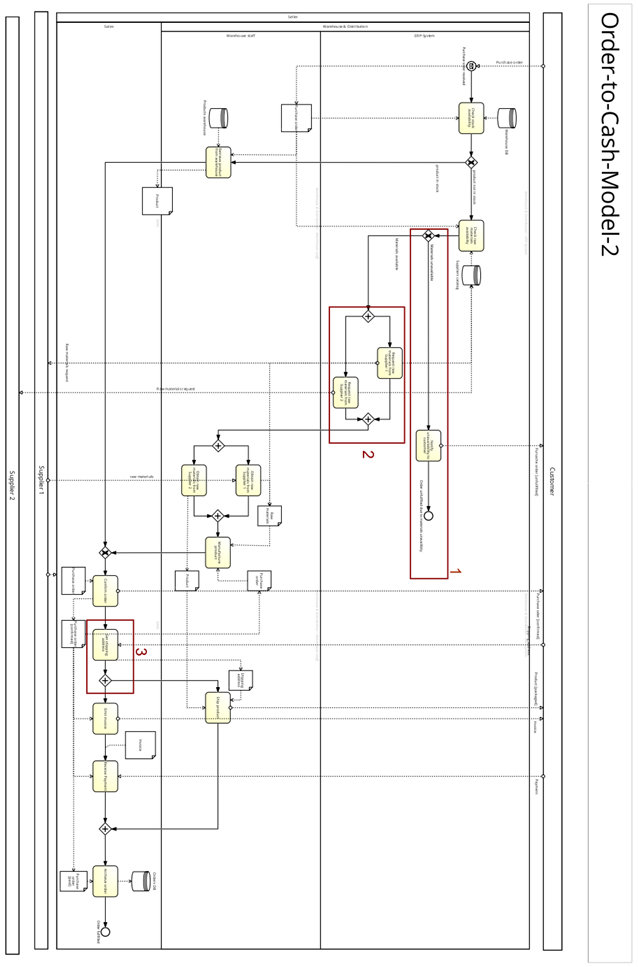
\includegraphics[height=23cm]{includes/p2_bpmn.png}}
        \caption{BPMN: Process 2 (Changed)}
        \label{bpmn2}
    \end{figure}
    In the previous page (\pageref{bpmn2}) you can see the customized process. The markers show the changes.\\
    The following adjustments were applied:
    \begin{enumerate}
        \item A new gateway was integrated. Here it is checked whether the raw materials are available at the suppliers. If this is not the case, a new end is reached and the customer is informed that the product is not available.
        \item Orders for raw materials have now been automated by the ERP system. A warehouse employee no longer must do this manually. For this purpose, the suppliers' databases were connected and automatic processes were started.
        \item The customer's delivery address is now entered directly by the sales staff, who also confirm the order. In addition, this changed the sequence and parallelism of the process steps.
    \end{enumerate}
\clearpage
%- - - - - - - - - - - - - - - - - - - - - - - - - - - - - - - - - - - - - - - - - - - - - - - - - - - - - - -
\chapter{Implementation}

    \section{Simulation}
    \begin{figure}[H]
        \centering
        \fbox{
\includegraphics[width=0.99\textwidth-2\fboxsep-2\fboxrule]{includes/blindbild.jpg}}
        \caption{Bildunterschrift}
        \label{soqu3}
        \small{Erstellt in Eigenarbeit in Anlehnung an \cite[see][]{us2020}}
    \end{figure}
    \blindtext (siehe Abbildung \ref{soqu3})

    \section{Data Transformation}
    \begin{table}[H]
        \begin{tabular}{p{0.29\textwidth}p{0.65\textwidth}}
            \textbf{Inhalt} & Jemand musste Josef K. verleumdet haben, denn ohne dass er etwas Böses getan hätte, wurde er eines Morgens verhaftet. "Wie ein Hund!" sagte er, es war, als sollte die Scham ihn überleben.\\
            \textbf{Inhalt} & Jemand musste Josef K. verleumdet haben, denn ohne dass er etwas Böses getan hätte, wurde er eines Morgens verhaftet. "Wie ein Hund!" sagte er, es war, als sollte die Scham ihn überleben.\\
            \textbf{Inhalt} & Jemand musste Josef K. verleumdet haben, denn ohne dass er etwas Böses getan hätte, wurde er eines Morgens verhaftet. "Wie ein Hund!" sagte er, es war, als sollte die Scham ihn überleben.\\
            \textbf{Inhalt} & Jemand musste Josef K. verleumdet haben, denn ohne dass er etwas Böses getan hätte, wurde er eines Morgens verhaftet. "Wie ein Hund!" sagte er, es war, als sollte die Scham ihn überleben.\\
            \textbf{Inhalt} & Jemand musste Josef K. verleumdet haben, denn ohne dass er etwas Böses getan hätte, wurde er eines Morgens verhaftet. "Wie ein Hund!" sagte er, es war, als sollte die Scham ihn überleben.\\
        \end{tabular}
        \caption{Tabellenunterschrift}
        \label{tabe3}
    \end{table}
    \blindtext (siehe Tabelle \ref{tabe3})

    \section{Double Machine Learning}
    \blindtext\footcite[see][1]{voli2020}
\clearpage
%- - - - - - - - - - - - - - - - - - - - - - - - - - - - - - - - - - - - - - - - - - - - - - - - - - - - - - -
\chapter{Conclusion}
    \blindtext
\clearpage